\documentclass[a4paper]{article}

\usepackage{graphicx}
\usepackage{url}
\usepackage{verbatim}

\title{Notes on PLC cost models}
\author{Kenneth Mackenzie}
\date{20th July 2020}

\begin{document}
\maketitle
\noindent This document contains some comments on the Plutus Core cost models
defined in \verb|language-plutus-core/budgeting-bench|.  The main purpose
of this was to look at the model for \verb|DivideInteger|, whose results
don't seem to fit the data very well; however I've got some more general
comments here regarding the models for the other arithmetic functions.

\subsection*{Current setup}  The directory \url{language-plutus-core/budgeting-bench}
contains a number of benchmarks for the standard Plutus Core built-in
functions; these are implemented in \verb|Bench.hs| (using the
Criterion benchmarking library) and can be run via (for example)
\verb|stack bench language-plutus-core:|\verb|language-|\verb|plutus-|\\ \verb|core-budgeting-bench|.  This runs the benchmarks
and saves the output in \verb|csvs/benching.csv|.  The file
\verb|models.R| contains R code to read the CSV file and convert the
contents into an R data frame.%%
\footnote{The headers in the CSV file are produced by Criterion and
  (slightly annoyingly) are not immediately suitable for input to R:
  some reformatting using regular expressions is required in
  \texttt{models.R}.  To work with the data, I found it easier to
  to do some reformatting using a text editor to modify the CSV
  file to a form that could be read directly into R.  Can we get Criterion
  to produce suitable output directly, or maybe provide a script to
  do the conversion for us?  It might be tricky to do the latter in a portable way though.}

There is also some code which applies R's \verb|lm| command to fit
linear models to the data for the various builtins.  The aim of this
is to find formulas which predict the execution time or memory
consumption of a builtin when provided with particular inputs.  The
\texttt{lm} function performs linear regression on multiple
explanatory variables (ie, input values).  This is more versatile than
might be expected: simple transformations allow you to fit models to,
for example, logarithmic or exponential data, and polynomial models
can be automatically fitted by performing simultaneous regression on
their coefficients.  The input to \texttt{lm} can include
\textit{model formulas} which allow you to easily specify the expected
form of a model, and \verb|models.R| contains such formulas for each
of the PLC builtins: \verb|lm| is then used to fit models using these
formulas, and the model can be examined to see how well it describes
the input data, and how suitable it would be for predicting actual
execution costs.

\paragraph{Benchmark inputs.}  All of the arithmetic functions (which
are the only functions considered here) take two arguments.  The
benchmarks run each function on every pair of numbers from the set
$\{3^{2^n}: 1 \leq n \leq 16\}$.  The largest number in this
set is approximately $4.15 \times 10^{31268}$, so the benchmarks are dealing
with numbers which are highly unlikely to occur in practice; however,
we have to set on-chain execution prices in such a way as to deter denial 
of service attacks, so it's worth looking at the behaviour over a large
range of inputs.

\paragraph{Input costs.}  One wouldn't expect the execution cost
of a typical arithmetic function to depend linearly on the value of the
input, but rather on the number of digits or bits.  PLC integers are
implemented as Haskell \verb|Integer|s, which in turn are implemented
using the C \texttt{GMP} library, and the size of an input is taken to
be the number of bits which \texttt{GMP} would be expected to use for the
input: more precisely, sizes are measured using the method
\verb|memoryUsage|, which for an integer $n$ is defined to be $(\log_2
|n|) / 60$, approximately the number of 8-byte words required to
represent the integer; for $3^{2^{16}}$ the memory usage is 1731.

\subsection*{Comments on the models}
I tried some alternative models on the data in \verb|benching.csv|,
which has execution times for all of the arithmetic functions and
integer comparisons.  The file contains figures for some very large
inputs, but I filtered out everything with a memory usage greater than
2000 to match what happens in \verb|models.R| and in the current
version of \verb|Bench.hs|.  The models mostly seemed perfectly
reasonable, apart from those involving division (see below), but I
did have some comments on the models for addition and multiplication.

For simplicity, I'm referring to the input variables as $x$ and $y$,
and the execution time as $z$.  In the actual benchmark output these
are \verb|x_mem|, \verb|y_mem|, and \verb|Mean|, but these are a bit
tricky to type.  I've also multiplied the times by $10^6$ to get
something more readable: this means that you should read times as
being in milliseconds.

\subsubsection*{\texttt{AddInteger}}
The model formula for \verb|AddInteger| is \texttt{z $\sim$ I(x+y)},
which is asking to fit \verb|z| as a linear function of
\verb|x+y|.\footnote{If you just have \texttt{z $\sim$ x+y} then R
  fits a model which is linear in both \texttt{x} and \texttt{y}: the
  \texttt{I} tells R to ``quote'' its argument to suppress this
  special interpretation of the formula.}  This isn't necessarily
what you'd expect: to add an $m$-bit integer and an $n$-bit integer
you'd need a maximum of $m+n+1$ bits (and a proportional amount of
work), so \texttt{z $\sim$ pmax(x,y)} might be more
reasonable.\footnote{ \texttt{pmax} gives you the pointwise maximum of
  two vectors or scalars, whereas \texttt{max} gives you the maximum
  element of a vector.  This always catches me out.}

I looked at these two models and got the following results:
\newpage
{\footnotesize
\begin{verbatim}
> summary (lm(z~I(x+y), f))

Call:
lm(formula = z ~ I(x + y), data = f)

Residuals:
    Min      1Q  Median      3Q     Max 
-5.4549 -0.2054  0.0862  0.3106  1.1595 

Coefficients:
             Estimate Std. Error t value Pr(>|t|)    
(Intercept) 1.410e+01  4.415e-02  319.33   <2e-16 ***
I(x + y)    3.581e-03  5.736e-05   62.44   <2e-16 ***
---
Signif. codes:  0 ‘***’ 0.001 ‘**’ 0.01 ‘*’ 0.05 ‘.’ 0.1 ‘ ’ 1

Residual standard error: 0.5846 on 254 degrees of freedom
Multiple R-squared:  0.9388,	Adjusted R-squared:  0.9386 
F-statistic:  3898 on 1 and 254 DF,  p-value: < 2.2e-16
\end{verbatim}
}

{\footnotesize
\begin{verbatim}
> summary (lm(z~pmax(x,y), f))

Call:
lm(formula = z ~ pmax(x, y), data = f)

Residuals:
     Min       1Q   Median       3Q      Max 
-0.80133 -0.19719 -0.01031  0.28908  0.85890 

Coefficients:
             Estimate Std. Error t value Pr(>|t|)    
(Intercept) 1.403e+01  2.719e-02   516.1   <2e-16 ***
pmax(x, y)  4.117e-03  3.952e-05   104.2   <2e-16 ***
---
Signif. codes:  0 ‘***’ 0.001 ‘**’ 0.01 ‘*’ 0.05 ‘.’ 0.1 ‘ ’ 1

Residual standard error: 0.3575 on 254 degrees of freedom
Multiple R-squared:  0.9771,	Adjusted R-squared:  0.977 
F-statistic: 1.085e+04 on 1 and 254 DF,  p-value: < 2.2e-16
\end{verbatim}
}  

For the version involving \verb|pmax| both the $R^2$ figures and the
residuals (the difference between the actual data and the predictions
given by the model) are slightly better (here the mean of the \verb|z|
values is about 15.64). Maybe we should use the \texttt{pmax} version
instead: it would be worth having a more careful look.


\subsubsection*{\texttt{MultiplyInteger}}
For \verb|MultiplyInteger|, the code in \verb|models.R| filters out the figures
when $x=0$ or $y=0$.  I'm not sure if this makes a lot of difference.

I tried a number of models here (\texttt{z $\sim$ x+y}, \texttt{z
  $\sim$ I(x+y)}, \texttt{z $\sim$ x*y}, \texttt{z $\sim$ I(x*y)})
and none of them seemed to be particularly good, at least in terms of
residuals (you would expect the first of these to be the natural one,
since the size of the product of two integers is the sum of the sizes
of the two integers, more or less).  The smallest residuals came from
\texttt{z $\sim$ x*y}, with a minimum residual of -330.82 and a
maximum of 207.38 (positive means that the model gives and
underestimation, negative; given that the maximum $z$-value is about
1495, this is quite a big difference.  I think that the problem here
may just be that the data isn't very linear.
Figure~\ref{fig:mul-plot-large} shows a three-dimensional view of the
data, and it's noticeably curved.

\begin{figure}[!ht]
\centering
  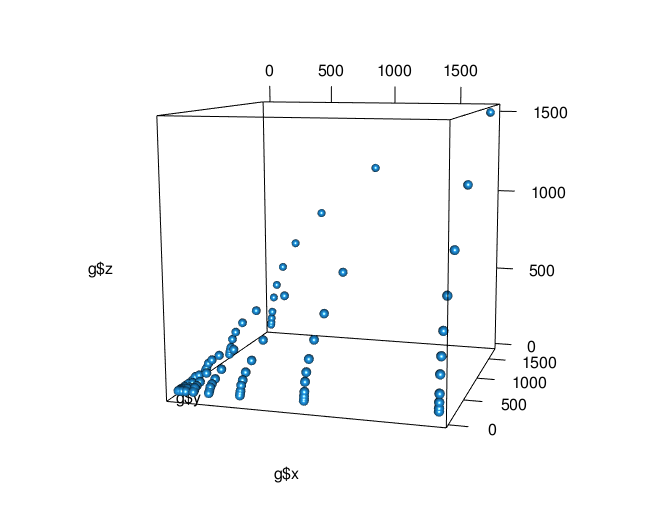
\includegraphics[width=0.8\textwidth]{figures/mul-large.png}
  \caption{Execution times for \texttt{MultiplyInteger}}
\label{fig:mul-plot-large}
\end{figure}

\paragraph{Smaller inputs.}
Recall however that the numbers here are extremely large: the maximum
inputs have over 32000 decimal digits.  I tried re-running the
benchmarks for \texttt{MultiplyInteger} with much smaller inputs,
specifically from the set $\{3*10^n+1234567: 1 \le n \le50\}$ (the
1234567 is an attempt to avoid peculiarities due to the numbers being
divisible by powers of 10, and hence divisible by powers of 2).

Figure~\ref{fig:mul-plot-small-1} shows a plot of execution times
against memory usage of inputs for the smaller inputs.  It's somewhat
difficult to see what's going on because the memory usage only takes
three values: 0,1, and 2.  To get a smoother view of the data,
Figure~\ref{fig:mul-plot-small-2} shows execution times plotted against
the logarithm of the actual input: the base-10 logarithm was used, but
this is proportional to the number of binary bits.  It is clear from
the second plot that the execution times are very uniformly
distributed with a few large random outliers.\footnote{
  In fact there's a small area possibly corresponding to inputs
  of at most 64 bits where the $z$-values are lower than all of the rest.}
The inputs here are up
to 50 digits long, which is still more than is likely to be used by
most legitimate calculations. This suggests that we may be able to get
away with a simpler cost most, where a flat fee is charged for small inputs
and punitive fees are charged for larger inputs.


\begin{figure}[!ht]
\centering
  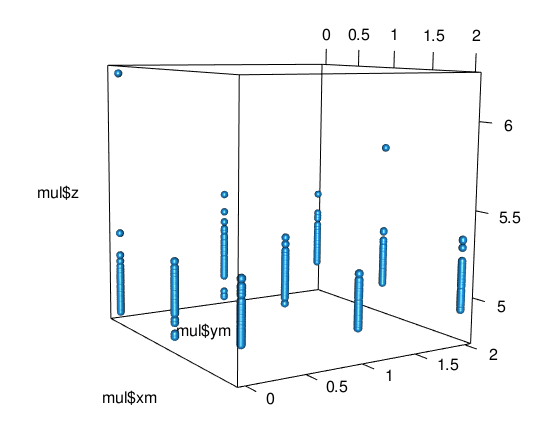
\includegraphics[width=0.8\textwidth]{figures/mul-small-1.png}
  \caption{Execution times for \texttt{MultiplyInteger}: small inputs, memory usage of inputs}
  \label{fig:mul-plot-small-1}
\end{figure}

\begin{figure}[!ht]
\centering
  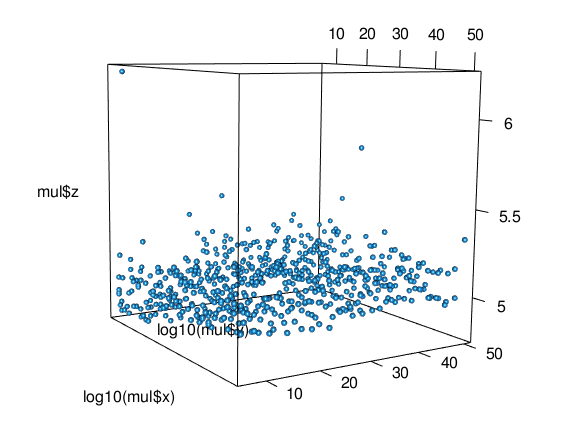
\includegraphics[width=0.8\textwidth]{figures/mul-small-2.png}
  \caption{Execution times for \texttt{MultiplyInteger}: small inputs, logarithm of inputs}
  \label{fig:mul-plot-small-2}
\end{figure}

\subsubsection*{\texttt{DivideInteger}}
It seems to be impossible to fit a sensible linear model to the data
for the \verb|DivideInteger| function (and also the
\verb|RemainderInteger|, \verb|QuotientInteger|, and \verb|ModInteger|
functions, which are all doing essentially the same thing).  Part of
the reason for this is that there's a sharp corner in the function: an
integer quotient $m/n$ is always zero (and cheap to compute) for
$n>m$, but can be expensive to compute for $m>n$.  However, even if we
filter out the inputs with $n>m$ it still doesn't seem to be possible
to find a sensible model.%%
\footnote{In \texttt{models.R}, this is done using \texttt{lm(Mean
    $\sim$ ifelse(x\_mem > y\_mem, I(x\_mem * y\_mem), 0)}; however, I
  think it's probably better to filter out the unwanted data
  \textit{before} trying to fit the model.}
Figure~\ref{fig:div-plot-Simon} shows a plot of the execution times
from \verb|benching.csv| (obtained on Simon's benchmarking machine)
and they're clearly a strange shape.  This isn't just due to random
fluctuations: Figure~\ref{fig:div-plot-kwxm} shows figures from a
re-run of the benchmark on my laptop: it's about 2.5 times faster, but
the data still has the strange shape.  I couldn't find any
transformation that makes things more linear, so I think trying to fit
a linear model may be a futile task (it's also difficult to find out
exactly how division is preformed in \texttt{GMP} (see below), so I can't see
what sort of formula we might expect).

\begin{figure}
\centering
  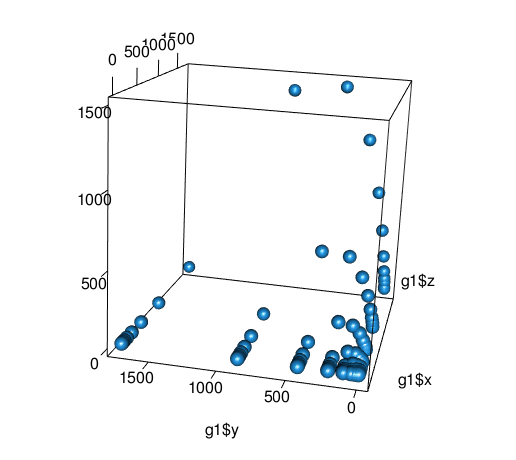
\includegraphics[width=0.8\textwidth]{figures/Simon.png}
  \caption{Execution times for \texttt{DivideInteger} on Simon's benchmarking machine}
  \label{fig:div-plot-Simon}
\end{figure}

\begin{figure}
\centering
  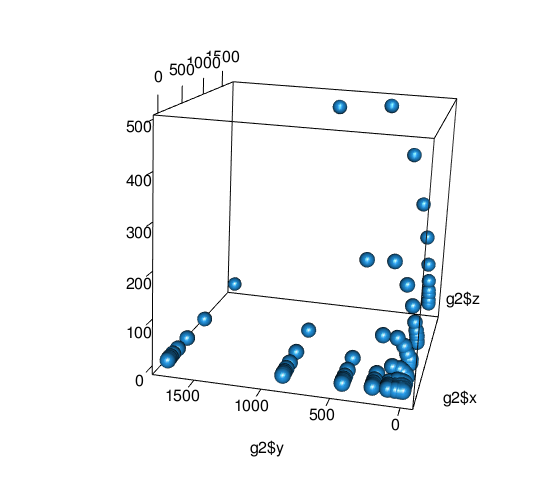
\includegraphics[width=0.8\textwidth]{figures/kwxm.png}
  \caption{Execution times for \texttt{DivideInteger} on Kenneth's laptop}
  \label{fig:div-plot-kwxm}
\end{figure}



However, I think we can avoid this problem in at least two different
ways.

\begin{itemize}
\item  I compared the execution times for \verb|DivideInteger| in
  \verb|benching.csv| with the execution times for multiplication of
  the same values and found that the execution time for division was
  never more than twice that for multiplication over the entire range
  of inputs.\footnote{At least for inputs restricted to have memory
    usage less than 2000; the file also contains data for inputs up to
    size 886375, which is over 16,000,000 decimal digits (!), and over this entire
    set division never took more than three times longer than
    multiplication.}
  Thus if we can find a good model for multiplication we could maybe get a safe bound
  for division just by saying that it should cost twice as much.
\item I also ran the division benchmark with the smaller inputs (up to
  50 decimal digits) mentioned in the section on
  \verb|MultiplyInteger| and got fairly uniform results: see
  Figure~\ref{fig:div-plot-small}. Thus again, charging a flat fee for small
  inputs might solve our problem.
  
\end{itemize}

\begin{figure}
\centering
  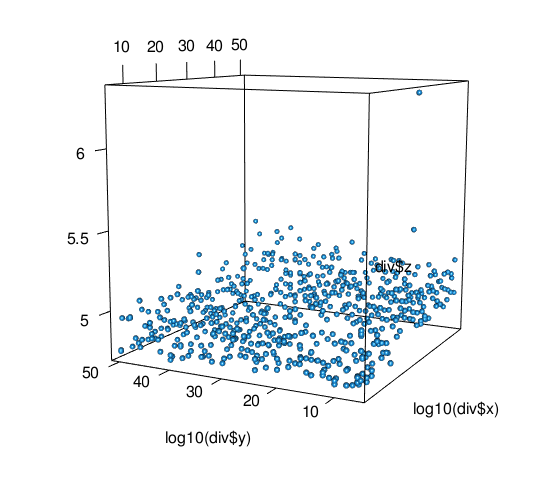
\includegraphics[width=0.8\textwidth]{figures/div-plot-small.png}
  \caption{Execution times for \texttt{DivideInteger}: small inputs, logarithm of inputs}
  \label{fig:div-plot-small}
\end{figure}

\subsubsection*{Other models}
I also looked at the models for functions for integer comparisons:
these seem well-behaved and unproblematic.

\subsection*{Remark on \texttt{GMP}}
Our integer functions are ultimately implemented via the \texttt{GMP} library.
It's quite difficult to follow exactly what's going on, but I think
the important parts of the code are all implemented in assembler: see
for example \url{https://gmplib.org/repo/gmp/file/tip/mpn}.  This
makes it rather difficult to see what the code is actually doing, and
the performance may be very device-dependent, so we may need different
cost models for different architectures.

\end{document}
